\chapter{Real-Time Rendering Definitions}\label{cha:definitions}

The terms such as for example surface, texture and material have various meanings depending on the context they are used in. Definitions from other scientific fields like engineering, chemistry and physics will not necessarily cover the same needs as in computer graphics. Defining a material as ``[\ldots] a substance that things can be made from.'' \cite{oxford2018dictionary} does not make a lot of sense for the virtual concept of material in computer graphics. Another issue is that even in computer graphics and across different 3D applications the terminology is often used inconsistently. Even throughout the same applications (e.g., \emph{UE4}) I found the use of the term material non-specific and referring to many different concepts. It is therefore essential for the clarity of this work to define the terminology used in this work first.


\section{Surface and Surface Area}\label{sec:surface}

In the present work \emph{surface} is used to describe the visual appearance of an object and the way it interacts with lights rather than the most outer area of an object in a geometrical sense. It refers to the different visual properties of an object like the age, history and usage of the castle wall (see chapter \ref{chahpter:introduction}).
To refer to its secondary meaning of the ``the outside part or uppermost layer of something'' \cite{oxford2018dictionary}, I will use explicitly the term surface area to make a clear distinction between both terms.


\section{Texture}\label{chapter:texture}
	A texture is often referred to as a color image that covers the surface area of an object, while, in practice, textures can contain all kinds of information influencing the shading equation. This work relies on the definition for texture defined by Thomas Akeninne-Möller et al. \cite[p.\,32--36]{akenine2008real}: ``[A texture] can be thought of as any large array of data.'' This statement already includes many properties that textures can influence. This array of data can contain the color data that is to be projected onto the mesh, but it can also contain all kinds of other shading information. Besides they are generally used to define a vast variety of surface properties by affecting the shading equation \cite[p.\,180--181]{akenine2008real} of a material.  Most of all bigger surface shading description is stored in this way. Joe Wilson \cite{wilson2015physically} gives examples of surface properties that are most often---but not exclusively---defined by textures:
	%
	\begin{description}
		\item[Diffuse:] These textures define the surface color and can be slightly different in name and stored information data depending on the application and shading model they are used for. The most commonly used names for diffuse textures in physically based shading are base color, diffuse and albedo. This work uses the term base color. 
		\item[Microsurface structure:] The two most commonly used maps to influence this property are roughness and glossiness maps. They basically define how rough or smooth a surface appears by influencing the shape of the specular reflection.
		\item[The amount of reflected light:] The most important texture inputs to influence this material property are metalness, specular and index of reflection \cite{wilson2015physically}.
	\end{description}
	%
	As mentioned before, textures are not always projected onto an object but can also be used as an object independent ``stand-alone data table'' \cite[p.\,462]{gregory2015game} as pointed out by Jason Gregory. Matt Pharr et al. \cite[p.\,597]{pharr2016physically} choose an even broader definition for a texture:
	
	\begin{itquote}
		[\ldots] a texture is a fairly general concept: it is a function that maps points in some domain (e.g., a surface’s $(u, v)$ parametric space or $(x, y, z)$ object space) to values in some other domain (e.g., spectra or the real numbers).
	\end{itquote} % \cite[p.\,597]{pharr2016physically}
	
	\begin{figure}
		\centering\small 
		\begin{tabular}{@{}ccc@{}}
			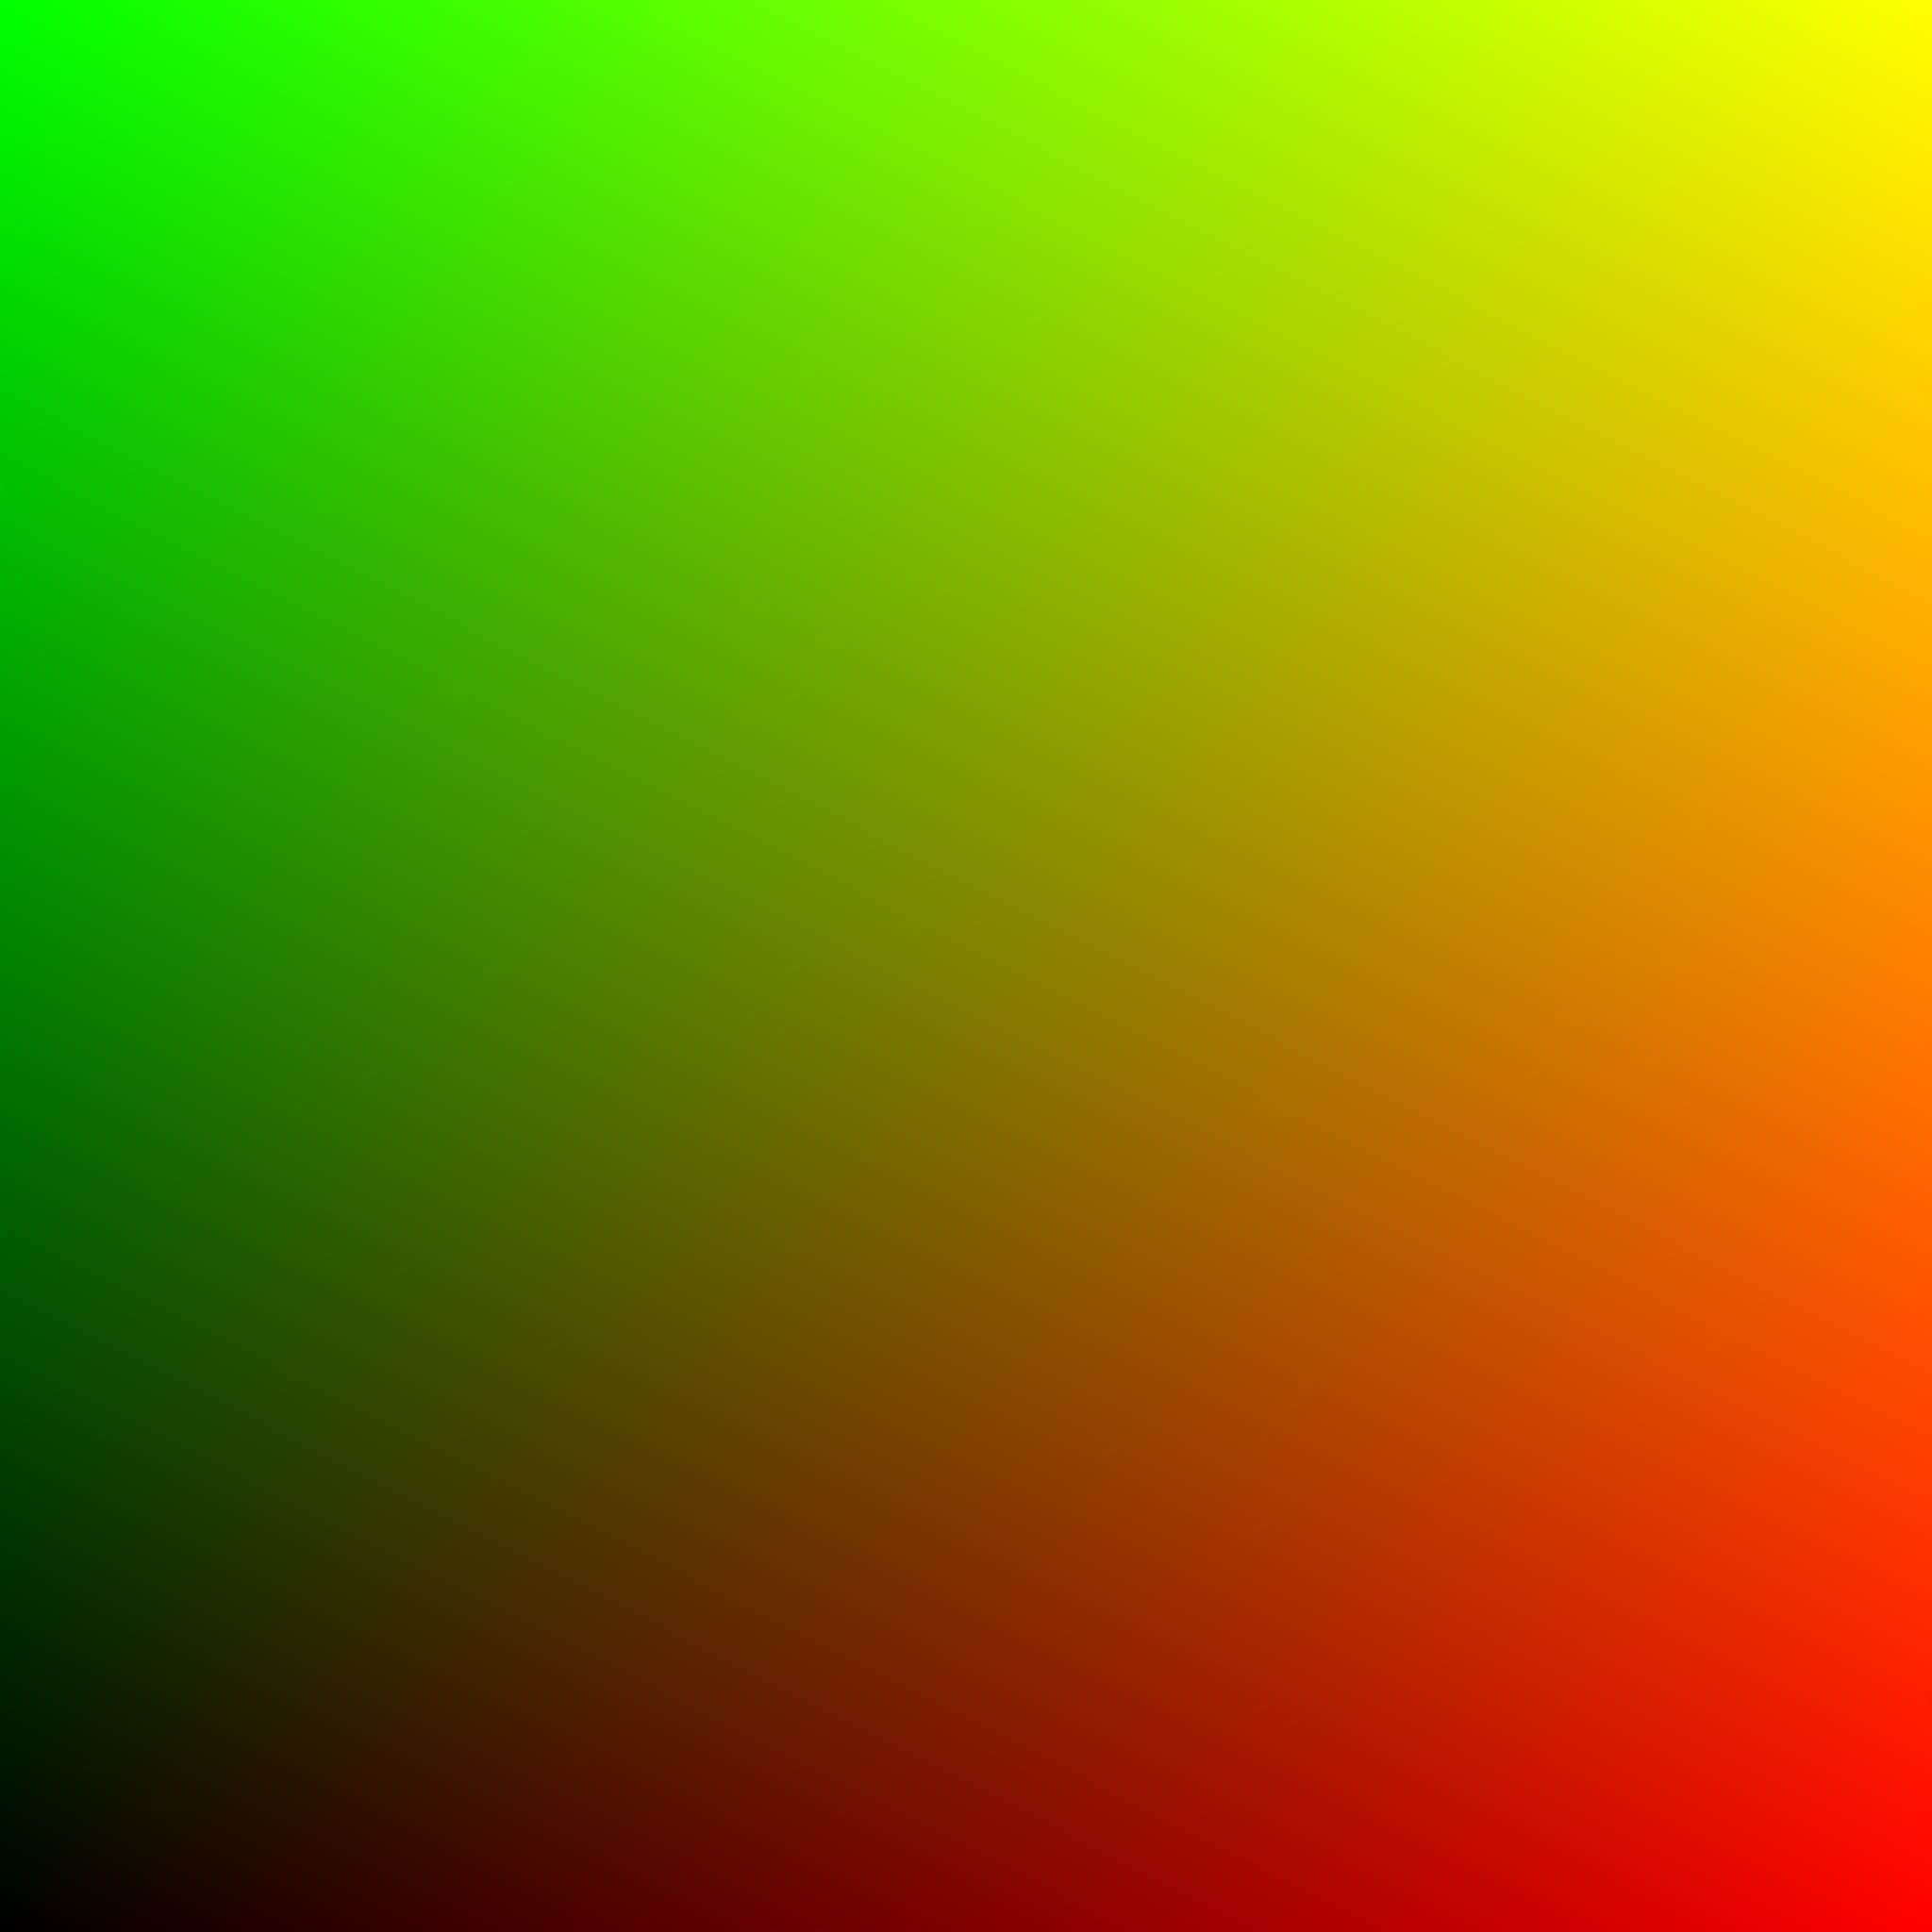
\includegraphics[width=0.3\textwidth]{images/02cha_01_TextureArrayOfData_uvCoordinates.jpg} &
			
\includegraphics[width=0.3\textwidth]{images/02cha_02_TextureArrayOfData_Perlin_Noise.jpg} &
			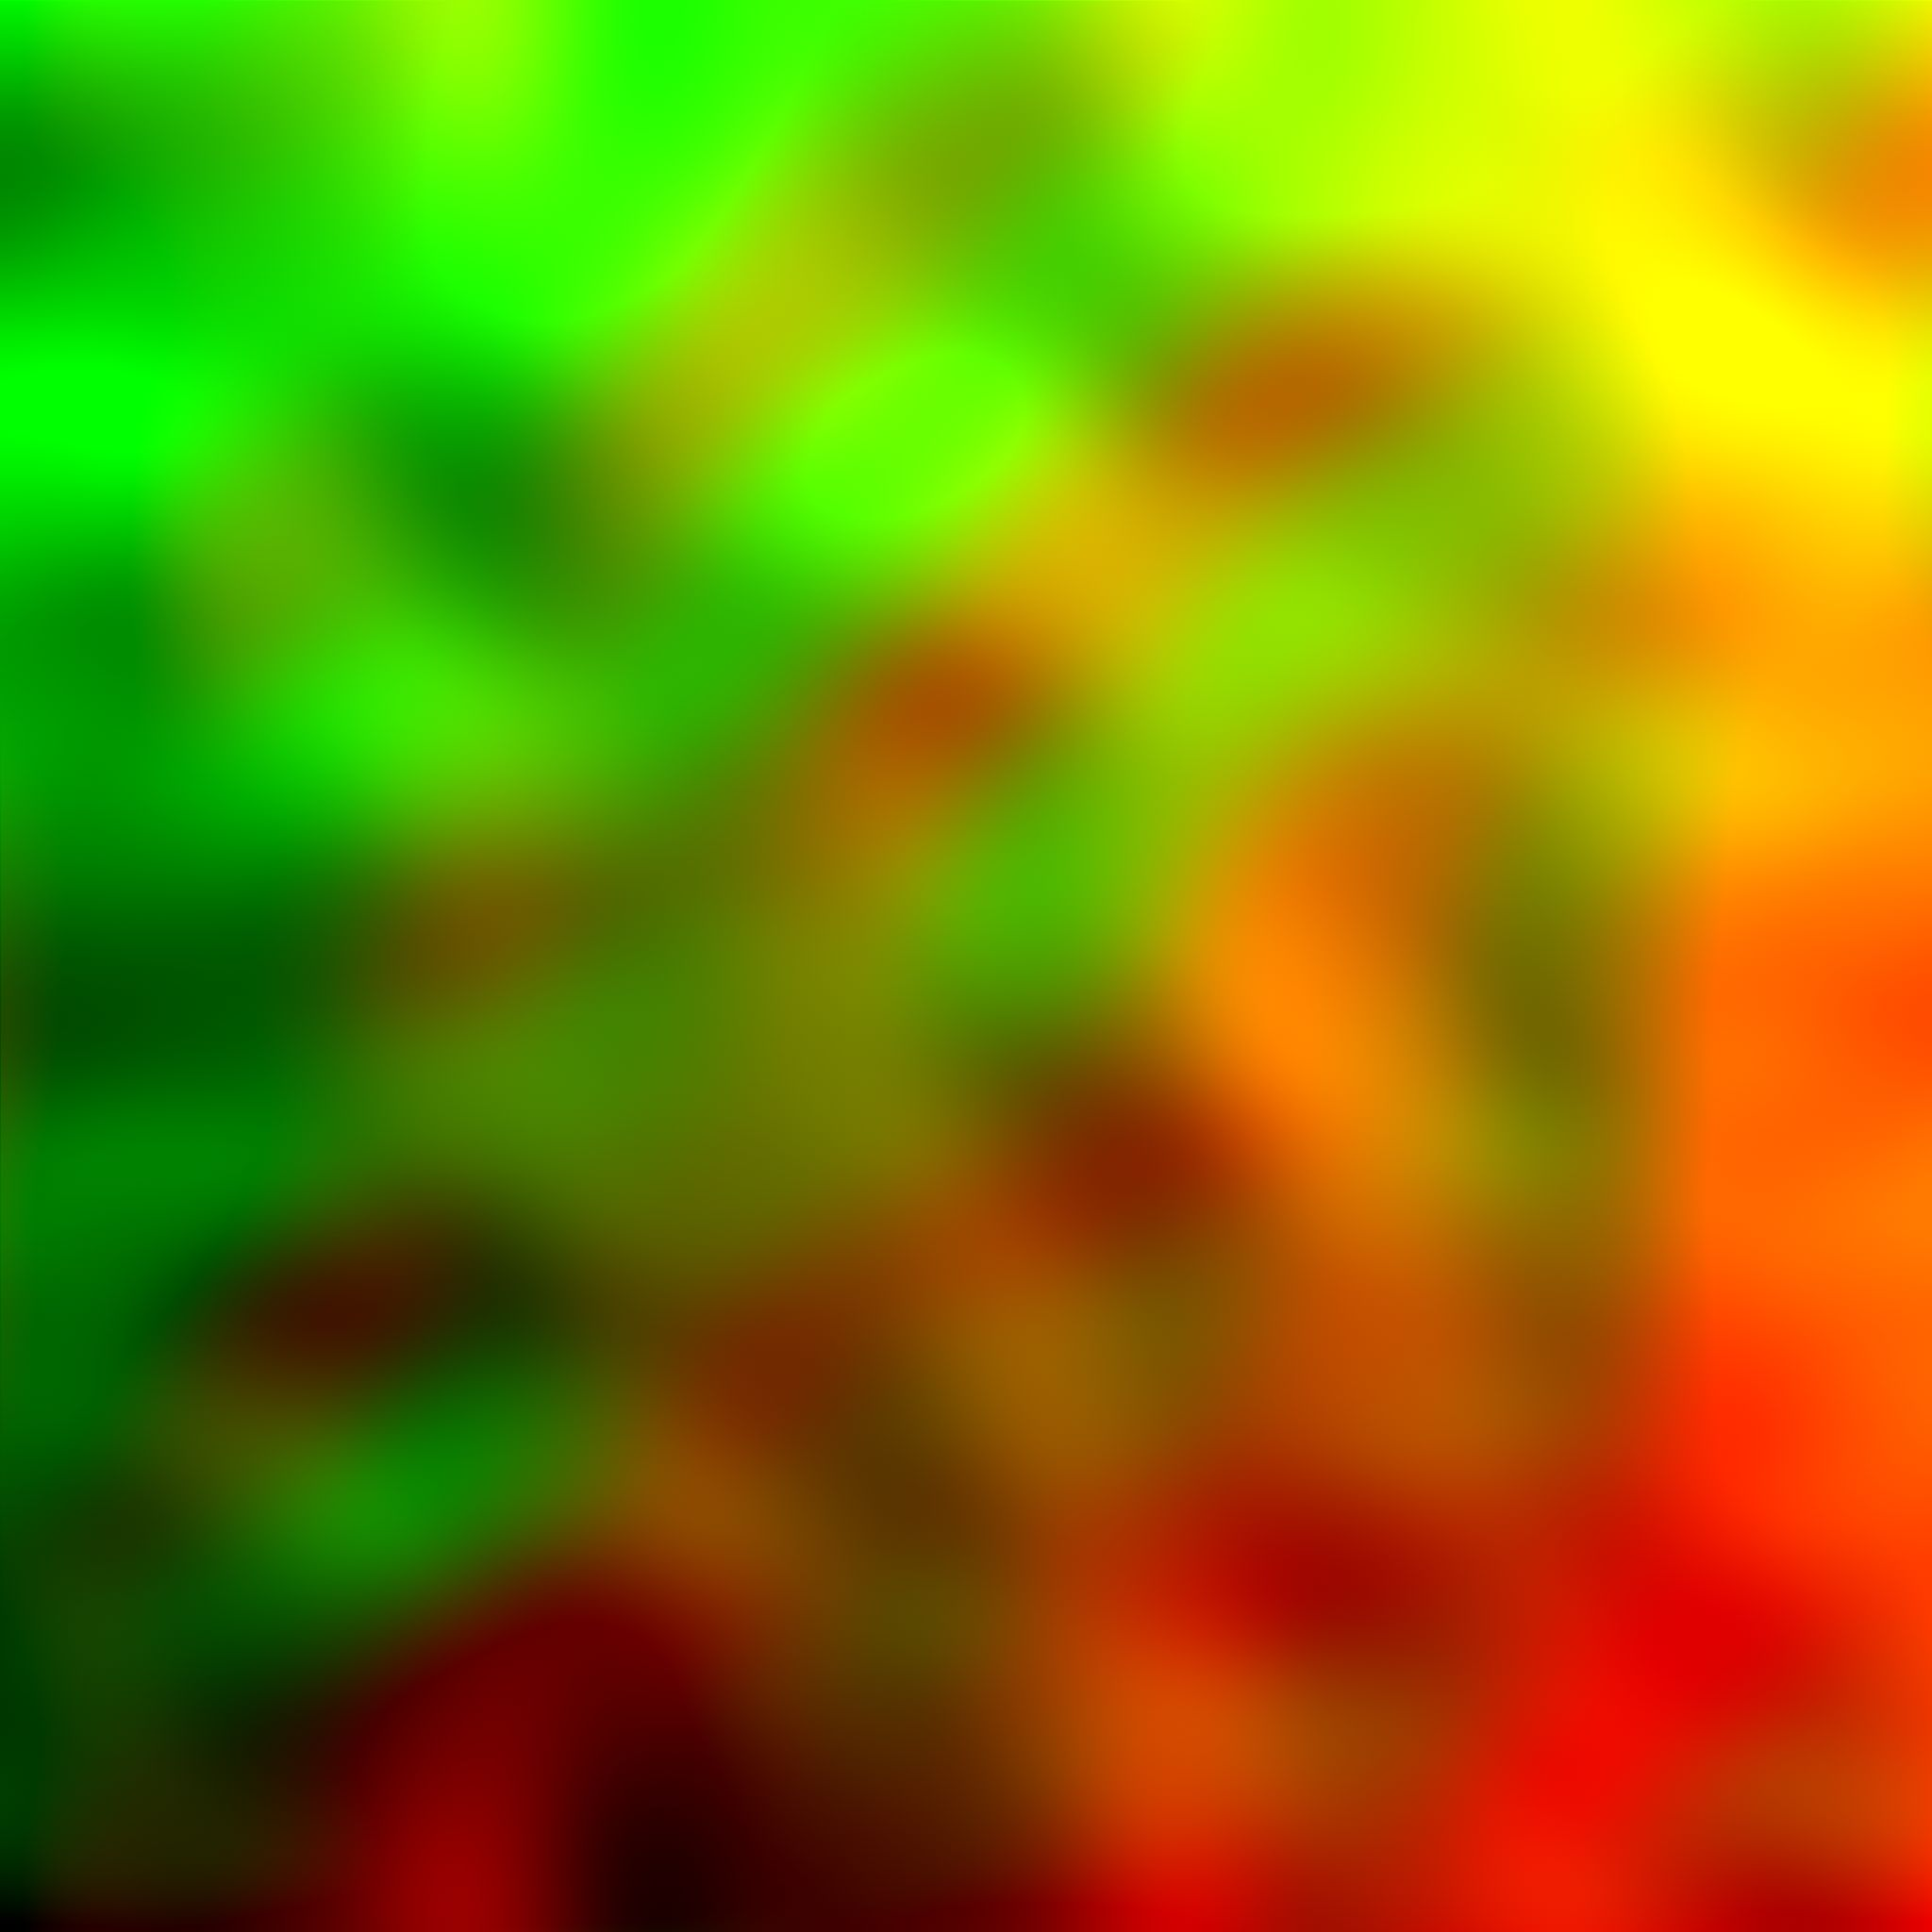
\includegraphics[width=0.3\textwidth]{images/02cha_03_TextureArrayOfData_Modified_UVs.jpg} \\	
			(a) & (b) & (c) 
		\end{tabular}	

		\caption{Using textures to manipulate UV coordinates. These images shows a less obvious example for using textures. The texture is not used to define a surface property but to manipulate the UV coordinates. Figure (a) shows a representation of the UV coordinates. The red and green value represent the U and V coordinates reaching from zero to one. Figure (b) shows a perlin noise texture that is used to manipulate the UV Coordinates within the shader. Figure (c) shows the manipulated UV coordinates that distorts the texture projection (e.g., base color, roughness) and can even be used to create animated shader effects. }
		\label{fig:textureExample}
	\end{figure}

\section{Material and Shading}\label{chapter:materials}

	The terms material and shader are closely connected with one another. The use of both terms seems inconsistent across different applications such as for example \emph{Unity} and \emph{UE4}. It is therefore especially important to define what those terms mean in the course of this work. Materials are defined by Akenine Möller et al. \cite[p.\,468]{akenine2008real} as follows:
	
	\begin{itquote}	
		A material is a complete description of the visual properties of a mesh. This includes a specification of the textures that are mapped to its surface and also various higher-level properties, such as which shader programs to use when rendering the mesh, the input parameters to those shaders and other parameters that control the functionality of the graphics acceleration hardware itself.
	\end{itquote} % \cite[p.\,468]{akenine2008real}

	The term shader does include all these shader programs: the input manipulation within the shader code and shading graphs. This definition also allows to give statements regardless of the underlying shading language and hardware. The terminology for texture, material and shader within \emph{Unity} applies to this work. A shader within \emph{Unity} is defined as follows \cite{unity2017textureShaderMat}: 

	\begin{itquote}
		A Material specifies one specific Shader to use, and the Shader used determines which options are available in the Material.
	\end{itquote} % \cite{unity2017textureShaderMat}
	%
	This simplified definition of a shader will work for most parts within this work. Materials within \emph{UE4} are defined as follows in contrast the prior definition \cite{epic2017materialDef}:
	%
	\begin{itquote}		
		Materials are defined by a set of states that control how the material is rendered (blend mode, two sided, etc.) and a set of material inputs that control how the material interacts with the various rendering passes (Base Color, Roughness, Normal, etc.).
	\end{itquote} % \cite{epic2017materialDef}
	
	Materials within \emph{UE4} can perform both functionalities of a shader as well as the model specific descriptions---see definition above. An \emph{UE4} material can contain certain descriptions of how to evaluate the shader equation, but it can also be applied to a mesh directly. 
	To avoid further confusion, this work will use a strict separation between \emph{UE4} material instances and materials. \emph{UE4} materials are strictly used as shaders. The material instances, on the other hand, are used as materials and contain the object specific values and textures. This aligns with the distinction between shader and material found in \emph{Unity}. In terms of this work, \emph{UE4} materials will be strictly used and referred to as shaders while material instances as materials.	Other meanings for materials within this work are:
	\begin{description}
		\item [Base Material:] Base material refers to a distinctive part of a surface area that differs in its physical properties. In contrast to material container, it describes the visual and artistic categorization. A surface can be split into different generic base materials. These base materials can be used to recreate a similar surface to the initial reference, for example. The granularity of splitting a surface into different base materials is defined by the artist and the final purpose. In a complex environment a base material may refer to cobblestone as well as the more detailed individual layers such as stone, mud, pebbles etc.       
		\item [Material Container:]	A material container is a technical component of the material layering model (see chapter \ref{cha:partsOfLayeredShader}). In contrast to base material, it may not only represent the entire surface properties but may only contain technical parameters and variables.  
	\end{description}

\section{Summary}

The purpose of this chapter was to define the fundamental terminology for this work. This is necessary as terms like texture, material and shader are used inconsistently across  different applications and scientific fields. For the purpose of this work, a texture is defined as a stored set of data that can be mapped onto any object. It is used to influence the shader equation within the rendering process. A texture is therefore used to define certain surface properties like color, light interaction, blending mask or texture mapping independent lookup tables.\footnote{Lookup tables represent arrays of data. They are used in computer graphics to avoid heavy computation and use stored data with array indexing operations instead \cite{wiki2018LookupTable}.} 
A shader defines which parameters are available within a material. Every material has to specify one shader, while shaders can be assigned to an infinite amount of materials. The shader defines which parameters and textures are available within the material and how the material is processed and rendered on the GPU. A Shader defines the available inputs and the different shader programs used. Materials are directly applied to objects within the 3D scene and define the object specific inputs.    
